\subsection{Rationale functies}

\begin{definitie}
	Functievoorschrift

${\displaystyle f(x)=\frac{t(x)}{n(x)}}$ met $t(x)$ en $n(x)$ veeltermfuncties
en waarbij de graad van $n(x)$ minstens 1 is.
\end{definitie}

\begin{voorbeeld}
Voorbeelden van rationale functies: ${\displaystyle f(x)=\frac{x^{2}}{1+x}}$,
${\displaystyle f(x)=\frac{1}{x^{2}-1}}$, ${\displaystyle f(x)=\frac{3x-9}{x-3}}$

Voorbeelden van niet-rationale functies: ${\displaystyle f(x)=\frac{\sin x}{4x}}$,
${\displaystyle f(x)=\frac{2^{x}}{3x+5}}$, ${\displaystyle f(x)=\frac{\sqrt{x-1}}{x-3}}$

\end{voorbeeld}

\textbf{Grafische voorstelling}

Het domein van een rationale functie is $\mathbb{R\setminus}\textrm{\{nulpunten\:van\:de\:noemer\}}$.

\begin{definitie}
	Voorbeeld: het domein van ${\displaystyle f(x)=\frac{2x+2}{x-8}}$
is ${\displaystyle \mathbb{R}\setminus\{8\}}$
\end{definitie}

\textbf{Nulpunten}

De nulpunten van een rationale functie $f(x)$, zijn de nulpunten
van de teller, die niet de nulpunten van de noemer zijn.

De nulpunten van de noemer, noemen we de polen van de rationale functie
$f(x)$. Bij elke pool hoort een verticale asymptoot.

Punten die zowel nulpunt zijn van teller als noemer, geven aanleiding
tot de vorm $\frac{0}{0}$. Aangezien deze punten de noemer nul maken,
horen ze niet tot het domein, maar geven ook geen aanleiding tot een
asymptoot.


\textbf{Asymptoten}

\begin{enumerate}
\item De rechte $x=a$ is een \textbf{verticale asymptoot} (VA) van de
rationale functie $f(x)$ als en slechts als $a$ een nulpunt is van
de noemer en geen nulpunt van de teller.

\begin{equation*}
\lim_{\overset{x\rightarrow a}{<}}f(x)=\pm\infty\quad\textrm{of}\quad \lim_{\overset{x\rightarrow a}{>}}f(x)=\pm\infty \\
		\Rightarrow\:x=a\:\textrm{is een VA}
\end{equation*}

\begin{voorbeeld}
\ 
\begin{equation*}
f(x)=\frac{2x+1}{x-1}
\end{equation*}

Het nulpunt van de noemer, of de pool is $x=1$. Dit punt is geen
nulpunt van de teller. Dus, $x=1$ is een verticale asymptoot. De
functie $f(x)$ is niet gedefinieerd in het punt $x=1$.
\begin{equation*}
\lim_{\overset{x\rightarrow1}{<}}\left(\frac{2x+1}{x-1}\right)=-\infty\quad\textrm{en}\quad \lim_{\overset{x\rightarrow1}{>}}\left(\frac{2x+1}{x-1}\right)=+\infty
\Rightarrow\:x=1\:\textrm{is een VA}
\end{equation*}

\end{voorbeeld}

\item Een rationale functie $f(x)$ heeft een \textbf{horizontale asymptoot}
(HA) als en slechts als de graad van de teller \ensuremath{\le} graad
van de noemer.

\begin{equation*}
\lim_{x\to\pm\infty}f(x)=b
\Rightarrow\:y=b\:\textrm{is een HA}
\end{equation*}

\begin{voorbeeld}
\ 
\begin{equation*}
f(x)=\frac{2x+7}{4x^{2}+x+2}
\end{equation*}

De graad van de teller is 1, en de graad van de noemer is 2; dus deze
functie heeft een horizontale asymptoot.

\begin{equation*}
\lim_{x\to\pm\infty}\frac{2x+7}{4x^{2}+x+2}\overset{HGT}{=} \lim_{x\to\pm\infty}\frac{2x}{4x^{2}}=\lim_{x\to\pm\infty}\frac{1}{2x}=0
\displaystyle \Rightarrow\:y=0\:\textrm{is een HA}
\end{equation*}

\end{voorbeeld}

\item Een rationale functie $f(x)$ heeft een \textbf{schuine asymptoot}
(SA) als en slechts als de graad van de teller = graad van de noemer
+1.

\begin{equation*}
m=\lim_{x\to\pm\infty}\frac{f(x)}{x}\quad\textrm{en}\quad q=\lim_{x\to\pm\infty}\left[f(x)-mx\right]\Rightarrow\:y=mx+q\:\textrm{is een SA}
\end{equation*}

\begin{voorbeeld}
	\begin{equation*}
f(x)=\frac{x^{3}-4}{2x^{2}}
\end{equation*}

De graad van de noemer is 2, en de graad van de teller is (2+1=) 3,
dus deze functie heeft een schuine asymptoot.

\begin{eqnarray*}
m&=&\lim_{x\to\pm\infty}\frac{f(x)}{x}= \lim_{x\to\pm\infty}\frac{x^{3}-4}{2x^{3}}\overset{HGT}{=} \lim_{x\to\pm\infty}\frac{x^{3}}{2x^{3}}=\frac{1}{2}
\\
q&=& \lim_{x\to\pm\infty}\left[\frac{x^{3}-4}{2x^{2}}-\frac{1}{2}x\right]=\lim_{x\to\pm\infty}\left[\frac{x^{3}-4-x^{3}}{2x^{2}}\right]=0 \\
&&\Rightarrow\:y=\frac{1}{2}x\:\textrm{is een SA}
\end{eqnarray*}

\end{voorbeeld}

\begin{opmerking}
Als een functie $f(x)$ voor $x\rightarrow+\infty$ een
horizontale asymptoot heeft, kan ze voor $x\rightarrow+\infty$ geen
schuine asymptoot meer hebben. Hetzelfde geldt voor $x\rightarrow-\infty$.
\end{opmerking}
\end{enumerate}

\textbf{Tekenverloop}

Om het tekenverloop van een rationale functie te bepalen, moet het
tekenonderzoek van de teller en de noemer worden uitgevoerd. Het tekenverloop
van een constante, een lineaire en een kwadratische functie is gekend
(zie Module 2 sectie \ref{sec:eerste_tweede} en \ref{sec:vtf}).
Het teken van de rationale functie is het product van het teken van
de teller en het teken van de noemer.


\begin{voorbeeld}
Bespreek de rationale functie 
\begin{equation*}
f(x)=\frac{3x^{2}}{x^{2}-2}
\end{equation*}

\underline{Domein}

$\textrm{dom}f(x)=\mathbb{R}\setminus\{-\sqrt{2},\sqrt{2}\}$ want de noemer mag niet nul worden. Dit gebeurt als ${\displaystyle x^{2}-2=0}\Longleftrightarrow x=\pm\sqrt{2}$.

\underline{Nulwaarden}

Stap 1: Bepaal de nulpunten van de teller, deze zijn de nulpunten
van de functie $f(x)$. Dus $3x^{2}=0\Longleftrightarrow x=0$ .

$x=0$ is een nulpunt van de teller, maar niet van de noemer, dus
dit punt is een nulpunt van de functie $f(x)$.

Stap 2: Bepaal de nulpunten van de noemer, deze zijn de polen van
de functie $f(x)$. Bij elke pool hoort een verticale asymptoot.

$x=-\sqrt{2}$ en $x=+\sqrt{2}$ zijn de nulpunten van de noemer,
de functie $f(x)$ heeft dus twee verticale asymptoten.

\underline{Asymptoten}

Stap 3: Ga na of de functie een verticale asymptoot bezit. 

De rechte $x=-\sqrt{2}$ is een verticale asymptoot (VA) van de functie
$f(x)$ aangezien $-\sqrt{2}$ een nulpunt is van de noemer en geen
nulpunt van de teller is.

Hoe verloopt de functie $f(x)$ in de buurt van deze asymptoot:

\begin{equation*}
\textrm{LL}: \lim_{\overset{x\rightarrow-\sqrt{2}}{<}}\left(\frac{3x^{2}}{x^{2}-2}\right)=+\infty\quad\textrm{en}\quad \textrm{RL}:\lim_{\overset{x\rightarrow-\sqrt{2}}{>}}\left(\frac{3x^{2}}{x^{2}-2}\right)=-\infty
\Rightarrow x=-\sqrt{2} \text{is een VA.}
\end{equation*}

De rechte $x=+\sqrt{2}$ is een verticale asymptoot (VA) van de functie
$f(x)$ aangezien $+\sqrt{2}$ een nulpunt is van de noemer en geen
nulpunt van de teller is.

Hoe verloopt de functie $f(x)$ in de buurt van deze asymptoot:

\begin{equation*}
\textrm{LL}: \lim_{\overset{x\rightarrow\sqrt{2}}{<}}\left(\frac{3x^{2}}{x^{2}-2}\right)=-\infty\quad\textrm{en}\quad \textrm{RL}:\lim_{\overset{x\rightarrow\sqrt{2}}{>}}\left(\frac{3x^{2}}{x^{2}-2}\right)=+\infty \\
\Rightarrow x=+\sqrt{2} \text{is een VA.}
\end{equation*}


Stap 4: Ga na of de functie een horizontale asymptoot bezit. De functie
$f(x)$ heeft een horizontale asymptoot (HA) aangezien de graad van
teller (2\textsuperscript{de} graad) = graad van de noemer (2\textsuperscript{de}
graad).

\begin{equation*}
\lim_{x\to\pm\infty}\frac{3x^{2}}{x^{2}-2}\overset{HGT}{=} \lim_{x\to\pm\infty}\frac{3x^{2}}{x^{2}}=3 \\
\Rightarrow y=3\text{ is een HA}.
\end{equation*}

Stap 5: Ga na of de functie een schuine asymptoot heeft. De functie
$f(x)$ heeft voor $x\rightarrow+\infty$ en $x\rightarrow-\infty$,
al een horizontale asymptoot en kan bijgevolg geen schuine asymptoot
meer hebben.

\underline{Tekenverloop}

Stap 6: - Schrijf in \'e\'en tabel bovenaan alle nulpunten en alle polen
in stijgende volgorde. 

\begin{itemize}
\item Onderzoek het teken voor elke factor van $f(x)$ . 
\item Het teken van $f(x)$ is dan het product van deze tekens.
\end{itemize}

\begin{center}
	\begin{tabular}{c||cccccccc} 
$x$ &  & $-\sqrt{2}$ &  & $0$ &  & $-\sqrt{2}$ &  & ${\displaystyle \longrightarrow\mathbb{R}}$\\
\hline 
${\displaystyle 3x^{2}}$ & + &  & + & 0 & + &  & + & \\
\hline 
${\displaystyle x^{2}-2}$ & + & 0 & - & - & - & 0 & + & \\
\hline 
${\displaystyle f(x)=\frac{3x^{2}}{x^{2}-2}}$ & + & $\mid$ & - & 0 & - & $\mid$ & + & \\
\end{tabular}
\end{center}

\underline{Grafiek}

\gewonefiguur{width=10cm}{2_elem_rekenvaardigheden_B/inputs/vb_rat1}

%\begin{figure}
%\centering
%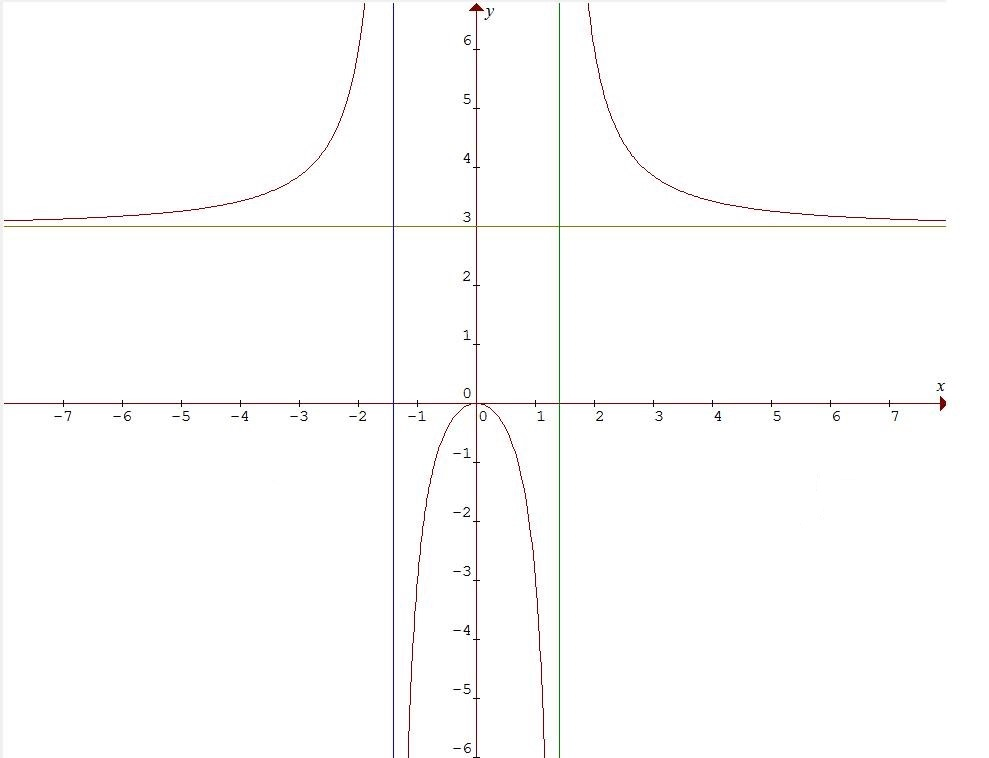
\includegraphics[scale=0.5]{2_elem_rekenvaardigheden_B/inputs/vb_rat1}
%\end{figure}


\end{voorbeeld}


\begin{ftonthoud}
	De grafiek en het tekenverloop van een rationale functie bepaal je
als volgt: $f(x)=\frac{t(x)}{n(x)}$ met $t(x)$ en $n(x)$ veeltermfuncties
en waarbij de graad van $n(x)$ minstens 1 is.

Het domein van een rationale functie is $\mathbb{R\setminus}\textrm{\{nulpunten\:van\:de\:noemer\}}$.

Stap 1: Bepaal de nulpunten van de teller, dit zijn de nulpunten van
de functie $f(x)$.

Stap 2: Bepaal de nulpunten van de noemer, dit zijn de polen van de
functie $f(x)$.

Stap 3: De rechte $x=a$ is een \textbf{verticale asymptoot} (VA)
van de rationale functie $f(x)$ als en slechts als $a$ een nulpunt
is van de noemer en maar geen nulpunt van de teller.

\begin{equation*}
\lim_{\overset{x\rightarrow a}{<}}f(x)=\pm\infty\quad\textrm{of}\quad \lim_{\overset{x\rightarrow a}{>}}f(x)=\pm\infty\quad\Rightarrow\:x=a\:\textrm{is een VA}
\end{equation*}


Stap 4: Een rationale functie $f(x)$ heeft een \textbf{horizontale
asymptoot} (HA) als en slechts als de graad van de teller \ensuremath{\le}
graad van de noemer. Maar hou wel rekening met het domein.

\begin{equation*}
\lim_{x\to\pm\infty}f(x)=b\quad\Rightarrow\:y=b\:\textrm{is een HA}
\end{equation*}

Stap 5: Een rationale functie $f(x)$ heeft een \textbf{schuine asymptoot}
(SA) als en slechts als de graad van de teller = graad van de noemer
+1. Maar hou wel rekening met het domein.

\begin{eqnarray*}
m= \lim_{x\to\pm\infty}\frac{f(x)}{x}\quad\textrm{en}\quad
q=\lim_{x\to\pm\infty}\left[f(x)-mx\right] \\
\Rightarrow\:y=mx+q\:\textrm{is een SA}
\end{eqnarray*}

Stap 6: Bepaal het tekenverloop
\begin{itemize}
\item Schrijf in \'e\'en tabel bovenaan alle nulpunten en alle polen in stijgende
volgorde. 

\item Onderzoek het teken voor elke factor van $f(x)$.

\item Het teken van $f(x)$ is dan het product van deze tekens.

\end{itemize}

\end{ftonthoud}
